\documentclass[../LogosReference.tex]{subfiles}
\begin{document}

% ============================================================================
% Section: Reflection Extension
% ============================================================================

\section{Reflection Extension}\label{sec:reflection}

The Reflection Extension enables first-person metacognitive reasoning through the \emph{I} operator.
Where the Agential Extension projects epistemic operators onto other agents, the Reflection Extension projects them onto the self, enabling perspectival distance from one's own beliefs, abilities, and goal-states.

\begin{remark}[Dependency]
This extension inherits from the Epistemic Extension in parallel with the Agential Extension.
Both apply the same epistemic apparatus: Agential projects outward onto other agents, Reflection projects inward onto self.
See the extension dependency diagram in \cref{sec:extension-dependencies}.
\end{remark}

% ------------------------------------------------------------
% Core Insight
% ------------------------------------------------------------

\subsection{Core Insight}\label{sec:reflection-insight}

The \emph{I} operator transforms direct modal expressions into self-aware epistemic stances.
Consider the difference between:

\begin{center}
\begin{tabular}{lll}
\toprule
\textbf{Expression} & \textbf{Reading} & \textbf{Epistemic Subject} \\
\midrule
$\mathsf{Mu}(\varphi)$ & ``It must be that $\varphi$'' & Implicit/absent \\
$\mathsf{I}(\varphi)$ & ``I believe that $\varphi$'' & Explicit (self) \\
\bottomrule
\end{tabular}
\end{center}

The direct expression commits the speaker without self-awareness; the self-aware expression registers the speaker as the epistemic subject.
This distinction follows Kaplan's character/content framework and Lewis's centered-worlds semantics.

% ------------------------------------------------------------
% Frame Extension
% ------------------------------------------------------------

\subsection{Frame Extension}\label{sec:reflection-frame}

The Reflection frame extends the Agential frame with:

\begin{center}
\begin{tabular}{ll}
\toprule
\textbf{Component} & \textbf{Description} \\
\midrule
Self-Index & Distinguished agent index $\mathsf{self} \in A$ \\
Self-Accessibility & Reflexive accessibility relation $R_{\mathsf{self}}$ \\
Self-Model & Function $\mathsf{SM}: W \to \mathsf{SelfState}$ \\
Commitment Register & Set $\mathsf{CR}(w)$ of self-ascribed propositions at $w$ \\
\bottomrule
\end{tabular}
\end{center}

The self-accessibility relation $R_{\mathsf{self}}$ satisfies:
\begin{itemize}
\item \textbf{Seriality (D)}: For all $w$, there exists $w'$ such that $(w, w') \in R_{\mathsf{self}}$
\item \textbf{Transitivity (4)}: Positive introspection: $\mathsf{I}(\varphi) \to \mathsf{I}(\mathsf{I}(\varphi))$
\item \textbf{Euclidean (5)}: Negative introspection: $\neg\mathsf{I}(\varphi) \to \mathsf{I}(\neg\mathsf{I}(\varphi))$
\end{itemize}

% ------------------------------------------------------------
% Truth Conditions
% ------------------------------------------------------------

\subsection{Truth Conditions}\label{sec:reflection-truth}

Given evaluation context $(\model, \history, x, \assignment, \vec{i})$, the primary $\mathsf{I}$ operator is defined by:

\begin{definition}[Truth Condition for $\mathsf{I}$]\label{def:reflection-truth}
$\model, \history, x, \assignment \vDash \mathsf{I}(\varphi)$ if and only if:
\begin{enumerate}
  \item For all $w'$ accessible via $R_{\mathsf{self}}$ from $\history(x)$:
        $\model, \history[w'/x], x, \assignment \vDash \varphi$
  \item $\varphi \in \mathsf{CR}(\history(x))$
\end{enumerate}
\end{definition}

\begin{remark}[Commitment Register Distinction]
The second condition distinguishes explicit self-attribution from mere truth across epistemic alternatives.
A proposition may hold at all worlds compatible with the agent's epistemic state without the agent having explicitly endorsed it.
The Commitment Register tracks which propositions the agent has actively self-ascribed,
capturing the difference between implicit epistemic commitment and explicit metacognitive awareness.
\end{remark}

% ------------------------------------------------------------
% Operators
% ------------------------------------------------------------

\subsection{Operators}\label{sec:reflection-operators}

\subsubsection{Self-Knowledge and Self-Belief}

\begin{center}
\begin{tabular}{lll}
\toprule
\textbf{Operator} & \textbf{Symbol} & \textbf{Reading} \\
\midrule
Metacognitive I & $\mathsf{I}(\varphi)$ & ``I judge/believe that $\varphi$'' \\
Self-Knowledge & $\mathsf{I}_K(\varphi)$ & ``I know that $\varphi$'' \\
Self-Belief & $\mathsf{I}_B(\varphi)$ & ``I believe that $\varphi$'' \\
Self-Uncertainty & $\mathsf{I}_?(\varphi)$ & ``I am uncertain whether $\varphi$'' \\
\bottomrule
\end{tabular}
\end{center}

\subsubsection{Ability Introspection}

\begin{center}
\begin{tabular}{lll}
\toprule
\textbf{Operator} & \textbf{Symbol} & \textbf{Reading} \\
\midrule
Self-Ability & $\mathsf{I}_{\mathsf{Can}}(\varphi)$ & ``I can bring about $\varphi$'' \\
Ability-Knowledge & $K_{\mathsf{self}}(\mathsf{Can}_{\mathsf{self}}(\varphi))$ & ``I know I can do $\varphi$'' \\
Limitation-Knowledge & $K_{\mathsf{self}}(\neg\mathsf{Can}_{\mathsf{self}}(\varphi))$ & ``I know I cannot do $\varphi$'' \\
\bottomrule
\end{tabular}
\end{center}

\subsubsection{Goal-Distance}

\begin{center}
\begin{tabular}{lll}
\toprule
\textbf{Operator} & \textbf{Symbol} & \textbf{Reading} \\
\midrule
Goal-Distance & $\mathsf{Dist}(G, n)$ & ``Goal $G$ is $n$ steps away'' \\
Goal-Progress & $\mathsf{Closer}(G)$ & ``I am getting closer to $G$'' \\
Goal-Achievable & $\mathsf{Achievable}(G)$ & ``Goal $G$ is achievable'' \\
\bottomrule
\end{tabular}
\end{center}

\subsubsection{Attributed Belief}

\begin{center}
\begin{tabular}{lll}
\toprule
\textbf{Operator} & \textbf{Symbol} & \textbf{Reading} \\
\midrule
Other's Belief About Self & $B_j(\mathsf{I}(\varphi))$ & ``Agent $j$ believes I believe $\varphi$'' \\
Other's Belief About Ability & $B_j(\mathsf{I}_{\mathsf{Can}}(\varphi))$ & ``Agent $j$ believes I can do $\varphi$'' \\
\bottomrule
\end{tabular}
\end{center}

\textsc{[Details pending development]}

% ------------------------------------------------------------
% Key Axioms
% ------------------------------------------------------------

\subsection{Key Axioms}\label{sec:reflection-axioms}

\begin{center}
\begin{tabular}{lll}
\toprule
\textbf{Axiom} & \textbf{Name} & \textbf{Schema} \\
\midrule
\textbf{I-T} & Veridicality & $\mathsf{I}_K(\varphi) \to \varphi$ \\
\textbf{I-4} & Positive Introspection & $\mathsf{I}(\varphi) \to \mathsf{I}(\mathsf{I}(\varphi))$ \\
\textbf{I-5} & Negative Introspection & $\neg\mathsf{I}(\varphi) \to \mathsf{I}(\neg\mathsf{I}(\varphi))$ \\
\textbf{I-D} & Consistency & $\neg\mathsf{I}(\bot)$ \\
\textbf{I-Commit} & Commitment Closure & $\mathsf{I}(\varphi) \to \mathsf{Register}(\varphi)$ \\
\bottomrule
\end{tabular}
\end{center}

\textsc{[Details pending development]}

% ------------------------------------------------------------
% Relationship to Agential Extension
% ------------------------------------------------------------

\subsection{Relationship to Agential Extension}\label{sec:reflection-agential}

The Reflection Extension inherits from the Epistemic Extension in parallel with the Agential Extension:

\begin{center}
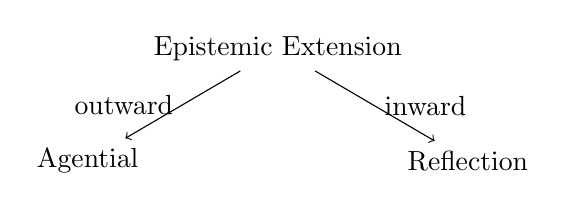
\begin{tikzpicture}[node distance=2cm, auto]
\node (epistemic) {Epistemic Extension};
\node (agential) [below left of=epistemic, xshift=-1cm] {Agential};
\node (reflection) [below right of=epistemic, xshift=1cm] {Reflection};
\draw[->] (epistemic) -- (agential) node[midway, left] {outward};
\draw[->] (epistemic) -- (reflection) node[midway, right] {inward};
\end{tikzpicture}
\end{center}

Both extensions apply the epistemic apparatus in different directions:
\begin{itemize}
\item \textbf{Agential}: $B_j(\varphi)$ -- ``Agent $j$ believes $\varphi$'' (modeling others)
\item \textbf{Reflection}: $\mathsf{I}(\varphi)$ -- ``I believe $\varphi$'' (modeling self)
\end{itemize}

\end{document}
